\documentclass{article}
\usepackage[utf8]{inputenc}
\usepackage[english]{babel}
\usepackage{geometry}
\usepackage{amssymb}
\usepackage{amsfonts}
\usepackage{dsfont}
\usepackage{float}
\usepackage{graphicx}
\usepackage{wrapfig}
\usepackage{mathtools}
\usepackage{bbm}
\usepackage{amsthm}
\usepackage{ifthen}
\usepackage{graphicx}
\usepackage{hyperref}
\usepackage{tcolorbox}
\usepackage[ruled,vlined]{algorithm2e}
\usepackage{tikz}

\usepackage{caption}
\usepackage{subcaption}

%%%%%%%% box %%%%%%%%
\definecolor{mycolor}{rgb}{0.122, 0.435, 0.698}% Rule colour
\makeatletter
\newcommand{\mybox}[1]{%
	\setbox0=\hbox{#1}%
	\setlength{\@tempdima}{\dimexpr\wd0+13pt}%
	\begin{tcolorbox}[colframe=blue,boxrule=0.5pt,arc=4pt,
		left=6pt,right=6pt,top=6pt,bottom=6pt,boxsep=0pt,width=\@tempdima]
		#1
	\end{tcolorbox}
}
%%%%%%%%





\DeclarePairedDelimiter{\ceil}{\lceil}{\rceil}

\newcommand{\ca}[1]{\mathcal{#1}}
\newcommand{\bb}[1]{\mathbb{#1}}
\newcommand{\p}{\mathbb{P}}
\newcommand{\evento}[1]{\left\{ \textit{``#1''} \right\}}
\newcommand{\comillas}[1]{``#1''}
\newcommand{\set}[1]{\left\{#1\right\}}
\newcommand{\parent}[1]{\left(#1\right)}
\newcommand{\parentCuad}[1]{\left[#1\right]}
\newcommand{\borel}{\ca{B}(\bb{R}^d)}
\newcommand{\Rd}{\bb{R}^d}
\newcommand{\R}{\bb{R}}
\newcommand{\infNorm}[1]{||#1||_\infty}
\newcommand{\condExp}[2]{\bb{E}(#1|#2)}
\newcommand{\ind}[1]{\mathbbm{1}_{#1}}
\newcommand{\esp}[1]{\bb{E}\barras{#1}}
\newcommand{\indep}{\rotatebox[origin=c]{90}{$\models$}}
\newcommand{\pe}{$(\Omega, \ca{F}, \p)\ $}
\newcommand{\vc}[1]{\langle #1 \rangle}
\newcommand{\gb}[1]{\overline{\widehat{#1}}}
\newcommand{\barras}[1]{\left| #1 \right|}
\newcommand{\integral}{\int_{t_i}^{t_{i+1}}}
\newcommand{\ug}[1]{\widehat{\ca{U}}_{#1}}
\newcommand{\vg}[1]{\widehat{\ca{V}}_{#1}}
\newcommand{\zg}[1]{\widehat{\ca{Z}}_{#1}}
\newcommand{\norm}[1]{\left\lVert#1\right\rVert}
\newcommand{\X}{\ca{X}}
\newcommand{\xscheme}[1]{X_{t_{#1}}^{\pi}}
\newcommand{\prom}[1]{\langle #1 \rangle}


\begin{document}
%%%
% Sacar el último plot. ASD
% Rellenar las otras partes. ASD
% Terminar el uml se forma simple.
% Crear una portada.


%%% Portada %%%
\begin{titlepage}
	\centering
	{\bfseries\LARGE Universidad De Chile \par}
	\vspace{1cm}
	{\scshape\Large Facultad de Ciencias Físicas y Matemáticas \par}
	\vspace{3cm}
	{\scshape\Huge LDA con datos de Twitter \par}
	\vfill
	{\Large  Javier Castro Medina\par}

	\vfill
	{\Large Abril 2021 \par}
\end{titlepage}
%%% Portada %%%
\newpage
%%%%

\section{Análisis Exploratorio}
En la primera parte del proyecto se realiza un proceso de adaptación a la librería \texttt{twint}, el formato de los datos que permite obtener y lo que podemos deducir de estos con un análisis exploratorio. Se decide buscar tweets en un radio de $10$ km con centro en las coordenadas de la facultad, que a simple vista coincide con el centro de la región Metropolitana. La razón de esta decisión es porque en esta región hay una población más grande y por lo tanto más probabilidad de encontrar cuentas de twitter. La presente sección se divide en dos partes, en la primera se mostrarán worclouds y en la segunda gráficos de la frecuencia de tweets diarios.
\subsection{Wordclouds}
	Acá mostramos dos hitos importantes, el primero es el estallido social del $18$ de octubre del $2019$ y el segundo es el día de la mujer del $2020$. El tercer wordcloud que se muestra corresponde a los tweets que contienen la palabra \comillas{piñera} durante el $2020$.
   	\begin{figure}[H]
   		\centering
   		\subfloat{
	   		\begin{minipage}[c][1\width]{0.45\textwidth}
	   			\centering
	   			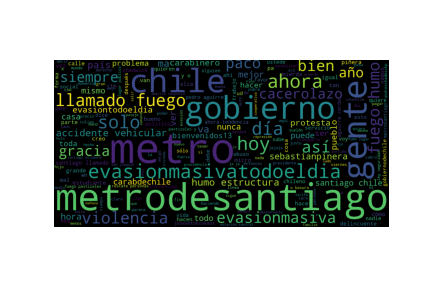
\includegraphics[width=\textwidth]{../imgs/wordcloud_santiago_estallido1.png}
	   			\caption{Tweets estallido social.}
	   		\end{minipage}
   		}
   		\hfill
   		\subfloat{
	   		\begin{minipage}[c][1\width]{0.45\textwidth}
	   			\centering
	   			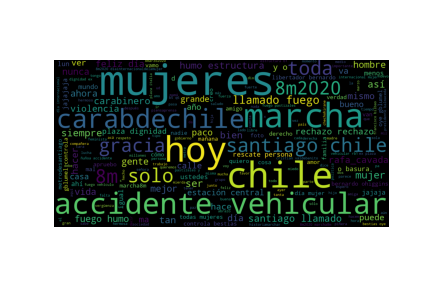
\includegraphics[width=\textwidth]{../imgs/wordcloud_santiago_8M.png}
	   			\caption{Tweets día de la Mujer.}
	   		\end{minipage}
		}
		\vfill
		\subfloat{
			\begin{minipage}[c][1\width]{0.45\textwidth}
				\centering
				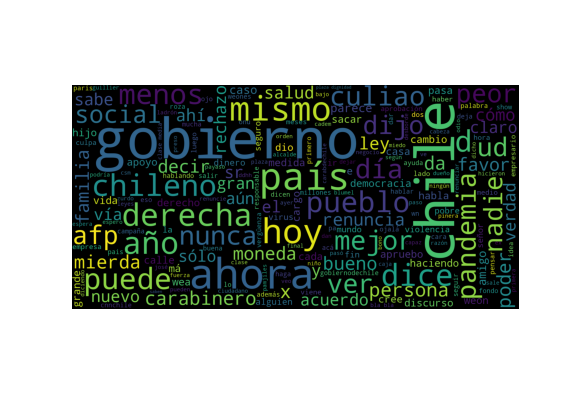
\includegraphics[width=\textwidth]{../imgs/wordcloud_santiago_pinera_2020.png}
				\caption{Tweets con la palabra \comillas{piñera} el $2020$.}
			\end{minipage}
		}
   	\end{figure}
\subsection{Series de tiempo}
Se expondrán series de tiempo relativas a la cantidad de tweets diarios que contengan cierta palabra clave. El primero tiene que ver con la pandemia.
\begin{figure}[H]
	\centering
	\subfloat{
		\begin{minipage}[c][1\width]{0.45\textwidth}
			\centering
			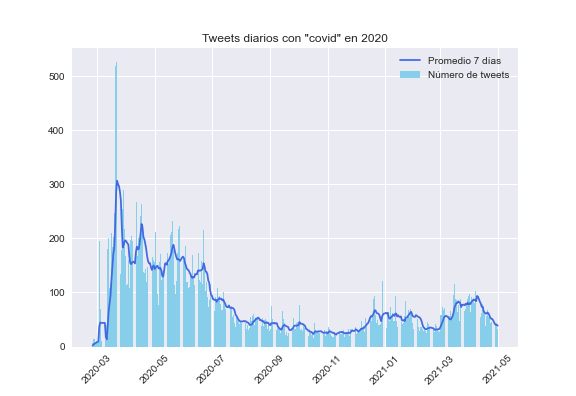
\includegraphics[width=\textwidth]{../imgs/serie_covid_2020.png}
			\caption{Tweets diarios con la palabra \comillas{covid}.}
		\end{minipage}
	}
	\hfill
	\subfloat{
		\begin{minipage}[c][1\width]{0.45\textwidth}
			\centering
			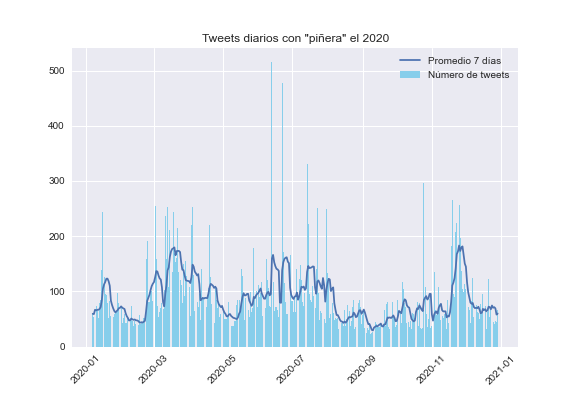
\includegraphics[width=\textwidth]{../imgs/serie_pinera_2020.png}
			\caption{Tweets diarios con la palabra \comillas{piñera}.}
		\end{minipage}
	}
\end{figure}

\newpage

\section{Latent Dirichlet Allocation}
	Este algoritmo cae en la categoría del \textbf{topic modelling} en la cual se busca, a partir de datos de texto, encontrar tópicos latentes. Para este modelo se necesita un set de palabras $V$ y una cantidad de tópicos $K$. Los tópicos se modelan como distribuciones sobre el conjunto de palabras $V$. Si bien este algoritmo tiene una fase generativa, su objetivo es calibrar parámetros $\alpha\in [0,1]^{K}$ y $\beta^{K\times V}$ optimizando una cota variacional. Estos parámetros determinan el modelo.\\
	
	Primero se hace un review a los datos mostrando distintas estadísticas asociadas a estos. Luego, se expone la limpieza y preprocesamiento que se realiza sobre el texto para dejarlo en condiciones de ser usado por el modelo y los métodos de la librería \texttt{gensim}. 
	
\subsection{Datos}
	Podríamos aplicar el modelo a todos los tweets de cierto espacio y tiempo pero se inclina por otro approach que es trabajar con los tweets de una cuenta en específico dado que el rango de temas o tópicos tocados por una cuenta es menor o más controlado que al trabajar con tweets de muchas cuentas. La cuenta que se escoge para partir es \texttt{@gabrielboric}, obtenemos sus tweets hasta junio del $2021$. Las características de este data set se pueden apreciar en las Figuras \ref{fig: boric_tweet_año} y \ref{fig: boric_tweet_2020}

	
	
	
 	\begin{figure}[H]
 		\centering
 		\subfloat{
 			\begin{minipage}[c][1\width]{0.45\textwidth}
 				\label{fig: boric_tweet_año}
 				\centering
 				\includegraphics[width=\textwidth]{../imgs/boric_tweet_año.png}
 				%\caption{Tweets por año.}
 			\end{minipage}
 		}
 		\hfill
 		\subfloat{
 			\begin{minipage}[c][1\width]{0.45\textwidth}
 				\centering
 				\label{fig: boric_tweet_2020}
 				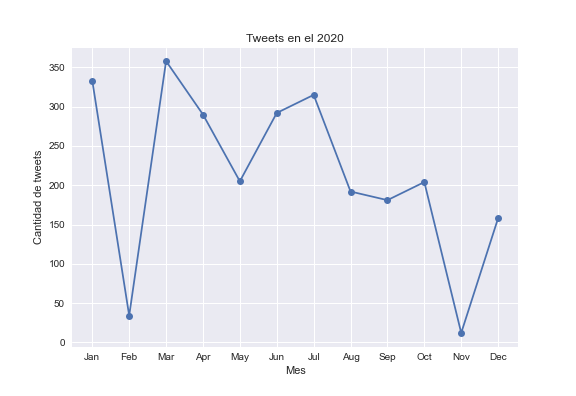
\includegraphics[width=\textwidth]{../imgs/boric_tweet_2020.png}
 				%\caption{Tweets por mes en el año $2020$.}
 			\end{minipage}
 		}
 		\caption{Tweets por año (izq) y por mes en el $2020$ (der).}
 	\end{figure}
 
	\begin{center}
		\begin{tabular}{ ||c|c|c|| } 
			\hline
			 & \textbf{Media} & \textbf{Min} \\ 
			\hline
			\hline
			Total & cell5 & cell6 \\ 
			$7$ días & cell8 & cell9 \\ 
			\hline
		\end{tabular}
	\end{center}
	
\subsection{Limpieza y preprocesamiento de datos}
	Los datos que se tienen disponible corresponden a tweets en formato de texto. El procesamiento de base o inicial que se realiza sobre este corpus corresponde a eliminar \textbf{stop words}, links, palabras de largo menor o igual a $3$, caracteres indeseables\footnote{Se eliminaron: \#, comas, signos de exclamación y pregunta, paréntesis y el signo igual.} y finalmente pasar todas las palabras a minúscula. El procesamiento anterior se realizará siempre y al inicio de todo código. Lo siguiente que se puede hacer es quitar palabras de baja frecuencia, sin quitar estas palabras el diccionario\footnote{Entendemos por diccionario al conjunto de todas las palabras utilizadas en el corpus} resultante tiene un tamaño de $35892$ palabras. En el gráfico a continuación muestra la cantidad de palabras resultantes al variar este parámetro.
	
	\begin{figure}[H]
		\centering
		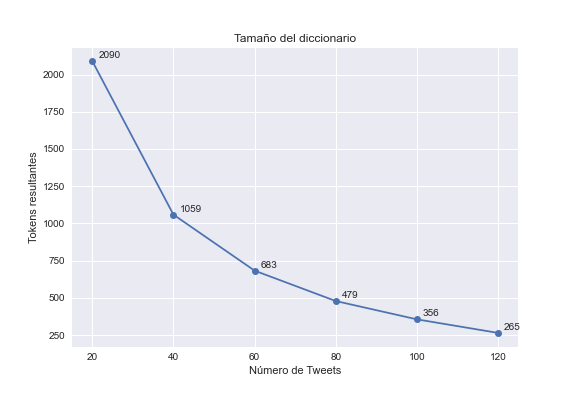
\includegraphics[scale=.5]{../imgs/no_below_len_dict.png}
		\caption{Tamaño del diccionario en función de la cantidad de tweets mínima a la que las palabras deben permanecer. Es decir, $y$ corresponde a las palabras que resultan al filtrar las que aparezcan en menos de $x$ tweets.}
	\end{figure}

	

	La siguiente etapa en el preprocesamiento es transformar los tweets en vectores. Para esto, a cada palabra del diccionario, digamos $V$, se le asigna un único índice de forma que el conjunto se palabras (o diccionario) se modela como $\set{1,...,|V|}$. Luego, cada tweet, entendido como una colección de palabras en $V$ de la forma $t=\set{v_1,...,v_n}$, se transforma en $\set{(v_1,r_1),...,v_n,r_n)}$ donde $v_i$ es el índice de la palabra en $V$ y $r_i$ la cantidad de veces que $v_i$ aparece en $t$. A continuación, un ejemplo de esto.
	
	\begin{figure}[H]
		\centering
		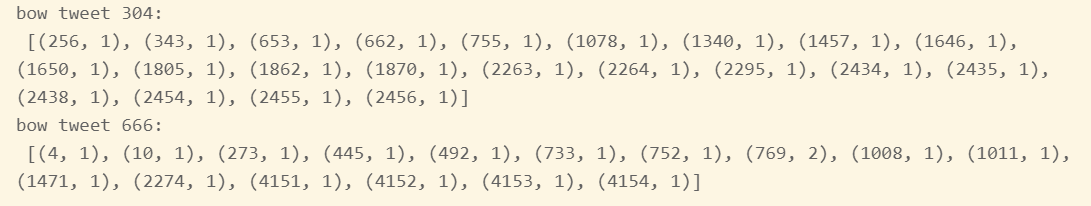
\includegraphics[scale=.5]{../imgs/bow_tweet_informe.png}
		\caption{Estado final de dos tweets escogidos al azar. Esta representación se conoce como \comillas{bow} (\textbf{bag of words}).}
		\label{fig: bow_example}
	\end{figure}
	
	\begin{remark}
		Notar que en los ejemplos que se muestran en la Figura \ref{fig: bow_example} la segunda componente de las tuplas es mayoritariamente $1$. Esto pasa porque el largo de cada tweet en el corpus es relativamente pequeño en comparación a otros set de datos como por ejemplo una colección de libros o notas periodísticas. Esto sugiere que esta variable no es muy decisiva en este contexto. 
	\end{remark}

	\begin{remark}
		Se decide dejar las palabras que hacen referencia a cuentas de Twitter, por ejemplo \texttt{@javier}. La razón de esta decisión es que la aparición de una cuenta en un tópico nos indica que tal persona es relevante para la cuenta sobre la que se está trabajando.
	\end{remark}

	\subsection{Aplicando el modelo}
	
	\textbf{Primera Iteración:} En la Figura \ref{fig: boric0_informe} se muestra el output de pedirle los tópicos al modelo.    
	
		\begin{figure}[H]
		\centering
		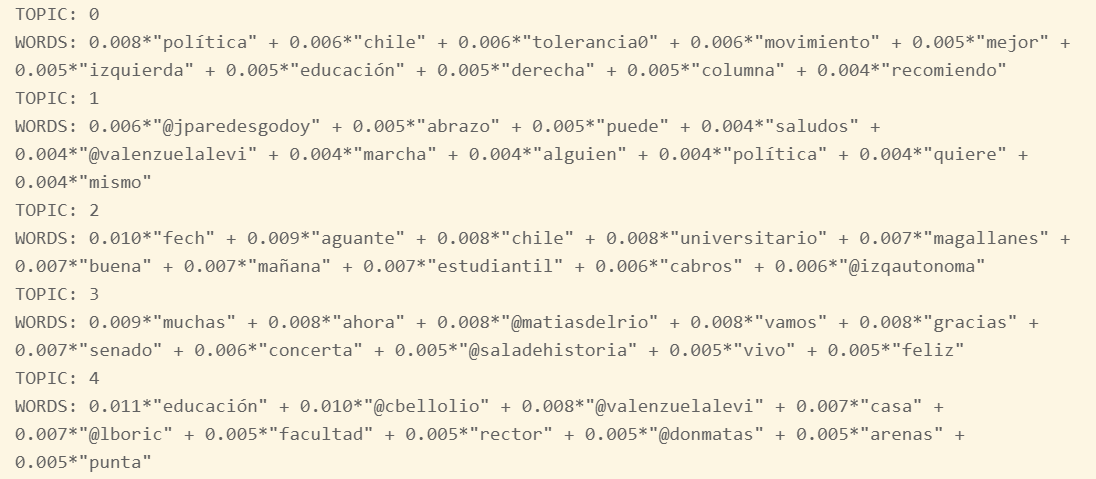
\includegraphics[scale=.5]{../imgs/boric0_informe.png}
		\caption{En esta iteración aplicamos el modelo fijando los parámetros al ojo y sin filtrar palabras poco frecuentes.}
		\label{fig: boric0_informe}
	\end{figure}
%\begin{thebibliography}{99}
	
\end{thebibliography}
\end{document}
